\section{Bottleneck \& Motivation}
\label{sec:motivations}

We observe severe GPU underutilization during agentic inference tasks.
Our investigation reveals that KV-Cache loading speed is the bottleneck due to the limited bandwidth of the single storage NIC on each node.
Analysis demonstrates that three decisive factors jointly cause this bottleneck, as discussed below.


First, agentic workloads exhibit high KV-Cache hit rates, which \emph{require more I/O and less computation}, thus creating a severe I/O bottleneck.
Agentic workloads are naturally long-context, short-append, and multi-turn.
On each turn, the GPU needs to read the KV-Cache of the entire context from persistent storage and perform prefill computation for appended tokens.
Our trace collected from representative coding tasks shows the mean number of rounds is 157, demonstrating the tendency of LLMs to engage in multi-turn interactions. The average context length is 32.7k, while the append length mean is only 429, which means a KV-Cache hit rate of 98.7\%. 
In such a scenario, the cache-compute ratio, defined as the ratio of KV-Cache to load and the computation needed, is approximately 22 GB/PFLOP for DeepSeek-V3.2 \cite{DeepSeekV32}, posing a significant bottleneck on storage bandwidth. 
Note that the KV-Cache size of DeepSeek MLA model is already highly optimized; for models with larger KV-Cache sizes (see \autoref{tab:cache-compute-ratio}), the situation is even worse. 
The ratio of DeepSeek-V3.2 is higher than DeepSeek-V3 \cite{deepseekv3}, benefiting from its sparse attention design, lowering computation demands.

\begin{table}[t]
  \centering
  \caption{\normalfont Cache-compute ratio with append length 429, across context lengths (16k--64k). KV-Cache data type defaults to FP8 unless specified.}
  \begin{tabular}{lc}
  \toprule
  Model & GB/PFLOP (16K--64K) \\
  \midrule
  % Gemma3-27B~\cite{gemmateam2025gemma3technicalreport} (FP16) & 1.0 \\
  Qwen2.5-32B~\cite{qwen2025qwen25technicalreport} (FP16) & 117-267 \\
  % DeepSeek-V3.2 27B~\cite{DeepSeekV32} & 70--184 \\
  GPT-OSS-120B~\cite{GPT-OSS} & 47--95 \\
  Qwen3-235B-A22B~\cite{yang2025qwen3technicalreport} & 39--60 \\
  DeepSeek-V3.2 660B~\cite{DeepSeekV32} & 13--36 \\
  % Kimi-K2-Base 1T~\cite{kimiteam2026kimik2openagentic} & 0.028 \\
  DeepSeek-V3 660B~\cite{deepseekv3} & 4.8--5.8 \\
  \bottomrule
  \end{tabular}
  \label{tab:cache-compute-ratio}
\end{table}

Second, the \emph{hardware evolution trend} is not well suited for agentic inference workloads.
In recent years, network bandwidth and HBM capacity have lagged behind the growth of GPU FLOPS, which drives us to run into memory and communication walls under agentic workloads.
As shown in \autoref{fig:motivation}, from NVIDIA Ampere to Blackwell, the I/O-compute ratio decreases by 14.4$\times$.
Low NIC bandwidth limits KV-Cache loading speed, making GPUs idle.
In addition, small HBM capacity limits the token batch size for GPU kernels \cite{ICLR24:FlashAttention2, FlashInfer, DeepGEMM, FlashMLA} to compute at the same time, hindering full utilization of compute units such as Tensor Core \cite{SOSP25:PrefillOnly}. % Small HBM capacity also limits the overlapping between computation and KV-cache transfers, which requires extra buffer, causing transfer latency to fall on the critical path.

Third, existing LLM inference systems exhibit severe \emph{storage network utilization imbalance} across different engine types. In prevalent PD-disaggregated systems, the KV-Cache for hit tokens is loaded exclusively by prefill engines directly from remote storage. This design centralizes all storage I/O pressure on the prefill-side SNICs, while the SNICs on decode engines remain largely idle. Consequently, the aggregate storage network bandwidth cannot be fully harnessed. % This static assignment of the KV-Cache loading role creates a fundamental and inefficient imbalance in storage network bandwidth utilization across engine types.

\begin{figure}[t!]
  \centering
  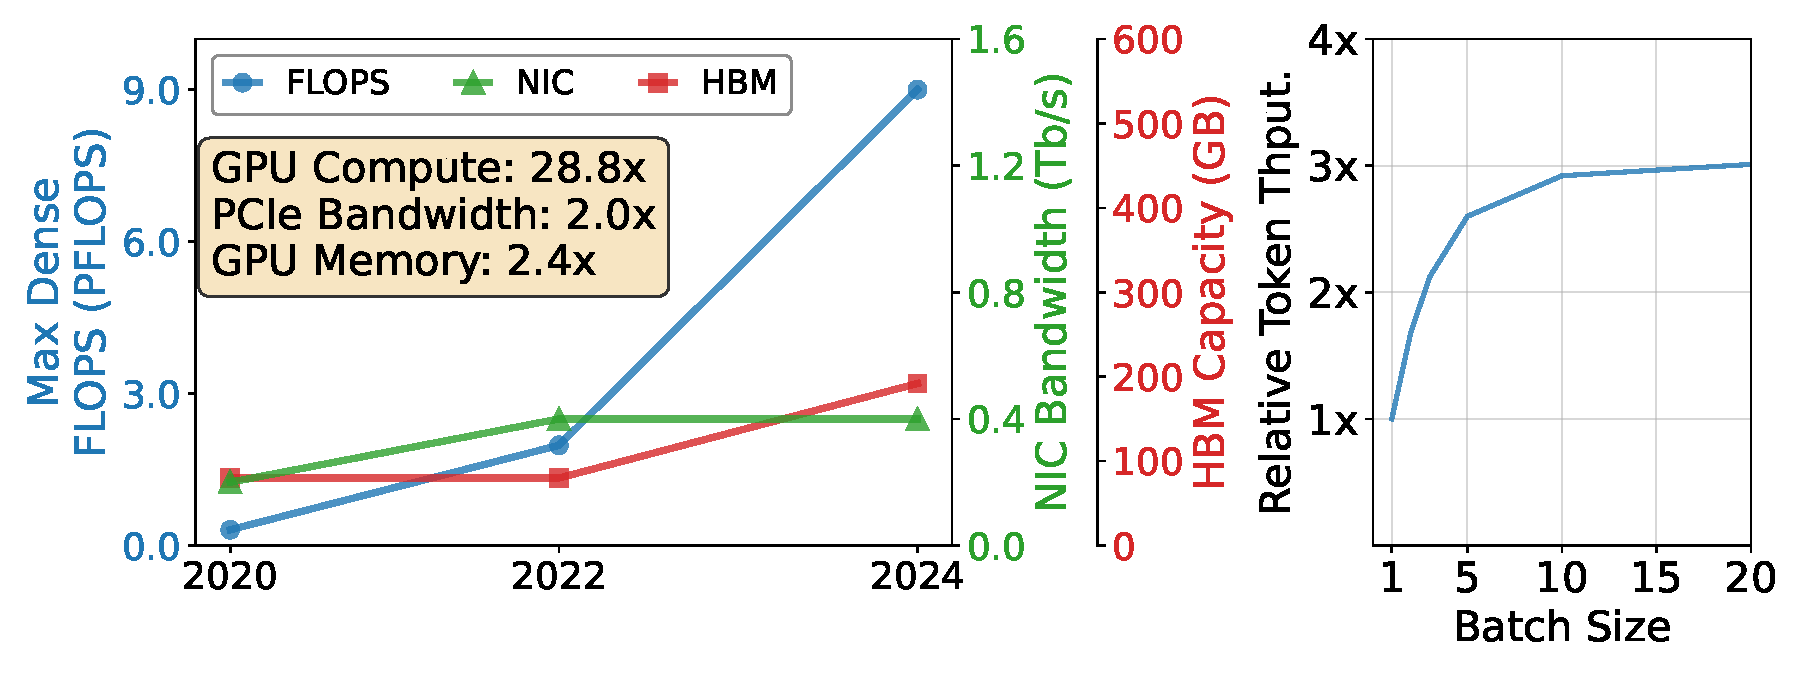
\includegraphics[width=1.05\linewidth]{figures/motivation.pdf}
  \vspace{-0.35in}
  \caption{\normalfont Left: Hardware trends of NVIDIA GPUs. Right: Relative token throughput with varying request batch size (each request has 30K context with 300 tokens appended).}
  \vspace{-0.2in}
  \label{fig:motivation}
\end{figure}


The above analysis demonstrates that the fundamental performance issue for agentic inference on PD-disaggregated architecture is the high I/O demand for KV-Cache retrieval and unbalanced storage network bandwidth utilization across inference engines. Meanwhile, we observe that the network traffic of the compute network, which has much larger aggregate bandwidth than the storage network, exhibits an intermittent pattern: collective operations used in model inference burst in sub-millisecond intervals. Therefore, an opportunity naturally emerges: we can utilize the SNIC bandwidth of decode nodes to load KV-Cache from storage, and transfer it back to the prefill nodes, utilizing the spare bandwidth of the faster compute network.
